%!TEX root = ./thesis.tex

\chapter{Error bound}
\label{cha:eb}


% ==============================================================================
\section{Error bound for Float}
% ==============================================================================
As posit is a widely used format, there already exists error bounds for floating point representation in the context of \glspl{spn} \cite{errorbound_float}. Using an absolute error bound would lead to very small quantity, therefore a relative error is used instead. This section report the method to compute error bound for floating point representation as described in \cite{errorbound_float}.

\todo[inline]{Is it clear enough that floating point comes from Nimish's paper ? To be discussed with Nimish. Value that are out of range for float are just discarded.}

\noindent Given that the goal is to use limit the number of bits used for a given representation, it may happen that a number of bits is not sufficient to represent all the values in a \gls{spn}. In this case, the number of bits is marked as \textit{out of range} and will be discarded.

\smallbreak

Given a number $f$, the encoded using a floating point representation is $\hat{f}$ with an absolute error of $\Delta f$ and a relative error of $\epsilon$ as described in Equation \ref{eq:float_error}.

\begin{equation}
	\tilde{f} = f \pm \Delta f = f \cdot \left(1 \pm \frac{\Delta f}{f} \right) = f \cdot (1 \pm \epsilon)
	\label{eq:float_error}
\end{equation}


% ------------------------------------------------------------------------------
\subsection{Encoding error}
% ------------------------------------------------------------------------------
The relative error for a floating point number can be computed based on the mantissa size ($ms$) as it is done is Equation \ref{eq:float_err_enc}

\begin{equation}
	\left| \frac{\Delta f}{f} \right| \leq 2^{-(ms+1)}
	\label{eq:float_err_enc}
\end{equation}


The relative error $\epsilon$ is then bounded by a value that does not depend on the value to be encoded, but depends on the number of mantissa bits (which is fixed). The only exception is zero, which can be encoded with a relative error equals to zero.

% ------------------------------------------------------------------------------
\subsection{Addition error}
% ------------------------------------------------------------------------------
Given $\epsilon$, the error of encoding a floating point number, a number $a$ with an accumulated relative error of $\epsilon_a$ and a number $b$ with an accumulated relative error $\epsilon_b$. A new error bound for the result of the addition of $a$ and $b$ can be computed through Equation \ref{eq:float_add_err}.

\begin{align}
\begin{split}
\hat{f} &= (\hat{a} + \hat{b}) \cdot (1 \pm \epsilon)\\
		&= (a \cdot (1 \pm \epsilon_a) + b \cdot (1 \pm \epsilon_b))\cdot (1 \pm \epsilon)\\
		&= (a + b + a \epsilon_a + b \epsilon_b) \cdot (1 \pm \epsilon) \\
		&= (a + b) \cdot \left(1 \pm \frac{a}{a + b} \cdot \epsilon_a \pm \frac{b}{a+b} \cdot \epsilon_b \right) \cdot (1 \pm \epsilon) \\
		&\leq (a+b) \cdot (1 \pm max(\epsilon_a, \epsilon_b)) \cdot (1 \pm \epsilon)\\
(1+\epsilon_f) &= (1 \pm max(\epsilon_a, \epsilon_b)) \cdot (1 \pm \epsilon)
\end{split}
\label{eq:float_add_err}
\end{align}

% ------------------------------------------------------------------------------
\subsection{Multiplication error}
% ------------------------------------------------------------------------------
Given $\epsilon$, the error of encoding a floating point number, a number $a$ with an accumulated relative error of $\epsilon_a$ and a number $b$ with an accumulated relative error $\epsilon_b$. A new error bound for the result of the addition of $a$ and $b$ can be computed through Equation \ref{eq:float_mult_err}.

\begin{align}
\begin{split}
\hat{f} &= \hat{a} \cdot \hat{b} \cdot (1 \pm \epsilon)\\
		&= a \cdot (1 \pm \epsilon_a) \cdot b \cdot (1 \pm \epsilon_b)\\
		&= a \cdot b \cdot (1 \pm \epsilon_a) \cdot (1 \pm \epsilon_b) \cdot (1 \pm \epsilon)\\
(1 \pm \epsilon_f) &= (1 \pm \epsilon_a) \cdot (1 \pm \epsilon_b) \cdot (1 \pm \epsilon)
\end{split}
\label{eq:float_mult_err}
\end{align}

% ==============================================================================
\section{Error bound for Posit}
% ==============================================================================
In this section, it is considered that a posit number has $N$ bits (without sign bit), $rs$ is the regime size (variable), $es$ is the number of exponent bits (fixed) and $ms$ is the number of mantissa bits.

As shown in Equation \ref{eq:rel_err}, the relative error for a posit representation can be expressed using the same method as for floating point (Eq. \ref{eq:float_err_enc}). Again, it is more interesting to compute the relative error since posit representation can encode very small and very big numbers.

\begin{equation}
	\hat{p} = p \pm \Delta p = p \cdot \left(1 \pm \frac{\Delta p}{p}\right) = p \cdot (1 \pm \epsilon)
	\label{eq:rel_err}
\end{equation}

% ------------------------------------------------------------------------------
\subsection{Encoding error}
% ------------------------------------------------------------------------------
Given a number which is in the bound of the posit representation, the maximum relative error that could occur is expressed by Equation \ref{eq:posit_enc_error}. This error represent the inability to encode one more fraction bit. The fraction size is represented by $fs$, $rs$ represents the regime size and $es$ the exponent size. $N$ is the number of bits of the posit representation.

\begin{equation}
	\left |\frac{\Delta p}{p} \right| \leq 2^{-(fs+1)} = 2^{-(N-min(rs+es, N)+1)}
	\label{eq:posit_enc_error}
\end{equation}


In contrast to floating point, this error highly depends on the number to be represented. It would be minimal for numbers around 1, and it would grows for high numbers and very small numbers (closer to 0). As it is shown in Figure \ref{fig:bfp}. The only exception is zero, which can be encoded with a relative error equals to zero.

\begin{figure}[!ht]
	\centering
	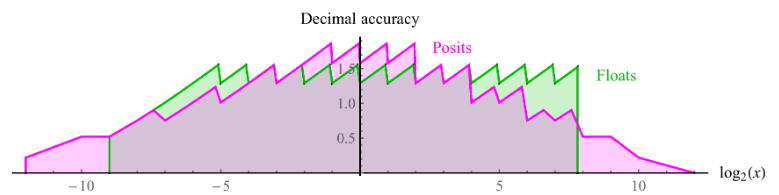
\includegraphics[width=0.9\linewidth]{../Images/decimal_accuracy.png}
	\caption{Image from \cite{bfp}. It shows how posit as a better accuracy for representing small numbers, and is able to represent very high numbers while floating point cannot.}
	\label{fig:bfp}
\end{figure}


% ------------------------------------------------------------------------------
\subsection{Addition error}
% ------------------------------------------------------------------------------
The error for every addition can be computed as it is done in Equation \ref{eq:posit_add_err}. In this case, $\epsilon$ represent the error performed while encoding the result of the operation. Therefore, it depends on the value of the number.

\begin{align}
\begin{split}
\hat{p} &= (\hat{a} + \hat{b}) \cdot (1 \pm \epsilon)\\
		&= (a \cdot (1 \pm \epsilon_a) + b \cdot (1 \pm \epsilon_b))\cdot (1 \pm \epsilon)\\
		&= (a + b + a \epsilon_a + b \epsilon_b) \cdot (1 \pm \epsilon) \\
		&= (a + b) \cdot \left(1 \pm \frac{a}{a + b} \cdot \epsilon_a \pm \frac{b}{a+b} \cdot \epsilon_b \right) \cdot (1 \pm \epsilon) \\
		&\leq (a+b) \cdot (1 \pm max(\epsilon_a, \epsilon_b)) \cdot (1 \pm \epsilon)\\
(1+\epsilon_f) &= (1 \pm max(\epsilon_a, \epsilon_b)) \cdot (1 \pm \epsilon)
\end{split}
\label{eq:posit_add_err}
\end{align}


% ------------------------------------------------------------------------------
\subsection{Multiplication error}
% ------------------------------------------------------------------------------
The error for every multiplication can be computed as it is done in Equation \ref{eq:posit_mult_err}. As for posit addition, $\epsilon$ depends on the result of the operation.

\begin{align}
\begin{split}
\hat{p} &= \hat{a} \cdot \hat{b} \cdot (1 \pm \epsilon)\\
		&= a \cdot (1 \pm \epsilon_a) \cdot b \cdot (1 \pm \epsilon_b)\\
		&= a \cdot b \cdot (1 \pm \epsilon_a) \cdot (1 \pm \epsilon_b) \cdot (1 \pm \epsilon)\\
(1 \pm \epsilon_p) &= (1 \pm \epsilon_a) \cdot (1 \pm \epsilon_b) \cdot (1 \pm \epsilon)
\end{split}
\label{eq:posit_mult_err}
\end{align}

% ==============================================================================
\section{Error bound for SPNs}
% ==============================================================================

% ------------------------------------------------------------------------------
\subsection{Floating point}
% ------------------------------------------------------------------------------

In order to compute the error bound for a \gls{spn}, the error must be computed for each node and be propagated up to the output. The error bound that is computed must be the worst case scenario. Therefore, there should not be any zero values since that is the only exception that can be encoded with a zero error.

By setting all the literals to one, and propagating the error up to the output of the \gls{spn}, we can then compute the error bound of floating point representation for a given network.

% ------------------------------------------------------------------------------
\subsection{Posit}
% ------------------------------------------------------------------------------
Error bound for posit require more work since the encoding error bound depends on the value which is encoded. Two cases must be taken into account: the maximum value of the \gls{spn}, and the minimum non-zero value of the \gls{spn}.

\paragraph{Error for maximum output value} This error can be computed by setting every input literal to one and propagate the error bounds up to the output. However, this error is rarely the biggest error since it is common to normalize the \gls{spn} at the end of the training (set maximum output to 1).

\paragraph{Error for minimum output value}

The smallest value is more difficult to compute since there are a lot of possible combination of inputs. Therefore, a trick is used to get an approximation of the minimum possible value of the \gls{spn}. This trick consist in setting every literal to one (as for the maximum value), and replacing every SUM node by MIN nodes. In this case, the output of the \gls{spn} may not be a valid set of literals. But the output is smaller than the minimum output for a valid set of literals.